\documentclass[11pt,letterpaper]{article}
\usepackage[T1]{fontenc}
\usepackage{lmodern}
\usepackage{graphicx}
\graphicspath{{./}{../}}
\providecommand{\pandocbounded}[1]{#1}
\usepackage{amsmath,amssymb,mathtools}
\usepackage[margin=1in,top=.85in,bottom=.85in]{geometry}
\usepackage{microtype}
\usepackage{enumitem}
\usepackage{titlesec}
\usepackage{needspace}
\usepackage[hidelinks]{hyperref}
\setlength{\parindent}{0pt}
\setlength{\parskip}{4.5pt plus 1pt minus 1pt}
\setlist{nosep,leftmargin=1.6em,topsep=4pt}
\setlength{\emergencystretch}{1.5em}
\allowdisplaybreaks[1]
\raggedbottom
\widowpenalty=10000
\clubpenalty=10000
\titleformat{\section}{\Large\bfseries}{}{0pt}{}
\titleformat{\subsubsection}{\normalsize\bfseries}{}{0pt}{}
\titleformat{\subsection}{\large\bfseries}{}{0pt}{}
\titlespacing*{\section}{0pt}{14pt}{8pt}
\titlespacing*{\subsubsection}{0pt}{9pt}{4pt}
\titlespacing*{\subsection}{0pt}{12pt}{6pt}
\newcommand{\tightlist}{\setlength{\itemsep}{0pt}\setlength{\parskip}{0pt}}
\hypersetup{pdftitle={Mathematical Analysis - Week
4},pdfsubject={MAT1011 Lecture 13-15, Tutorial 3 and Homework 3}}
\begin{document}
\begin{center}
{\LARGE Mathematical Analysis - Week 4\par}
\vspace{5pt}
{\large Lecture 13-15, Tutorial 3 and Homework 3\par}
\end{center}
\vspace{4pt}
\Needspace{10\baselineskip}
\section{Lecture 13}\label{lecture-13}

\Needspace{8\baselineskip}
\subsection{Inflection and curve
sketching}\label{inflection-and-curve-sketching}

\Needspace{5\baselineskip}
\textbf{Definition (slides' convention).} Inflection point: tangent
exists and strict concavity changes across the point. Vertical tangents
allowed. \(f''=0\) or undefined only gives candidates. \[
\begin{array}{c|c|c|c}
f&\text{concavity at }0&\text{tangent}&\text{inflection?}\\\hline
x^{5/3}&\text{down/up}&y=0&\text{yes}\\
x^{1/3}&\text{up/down}&x=0&\text{yes}\\
x^4&\text{up/up}&y=0&\text{no}\\
x^{2/3}&\text{down/down}&\text{cusp}&\text{no}
\end{array}
\]

\begin{center}
\begin{minipage}{\linewidth}
\centering
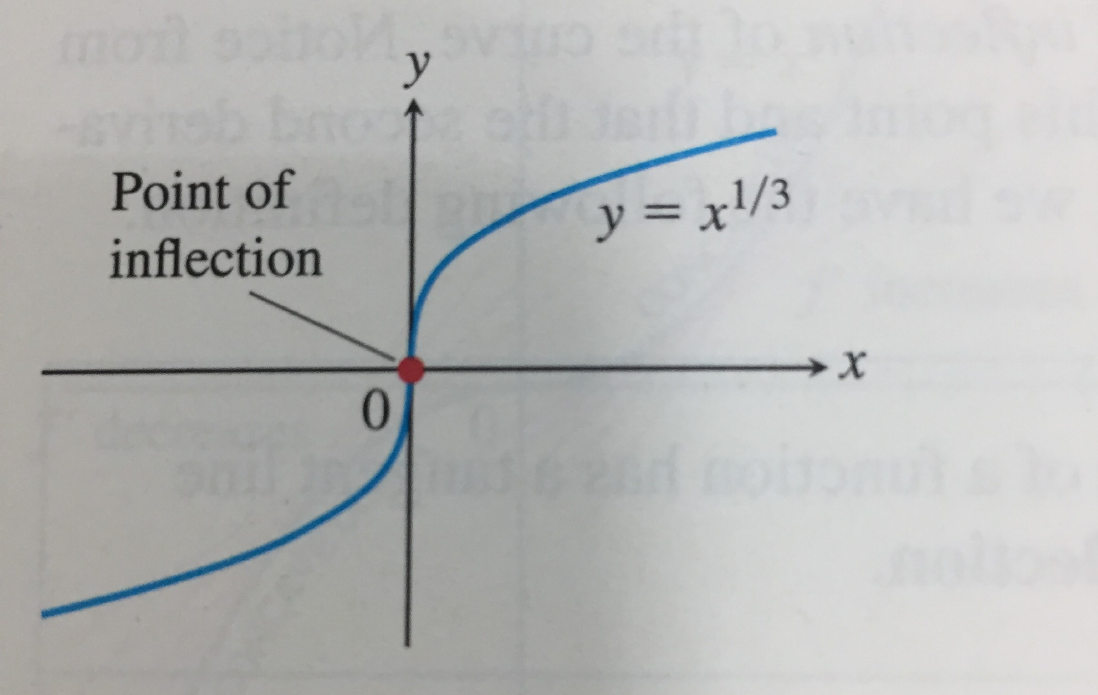
\includegraphics[width=0.3\linewidth,height=\textheight,keepaspectratio]{note-images/w4-cuberoot.png}\par
\vspace{3pt}
{\small \emph{Lecture 13, p.10.}\par}
\end{minipage}
\end{center}

\textbf{Ex.1.2.46.} \(f=(x+1)^2/(1+x^2)=1+2x/(1+x^2)\); domain
\(\mathbb R\). \[
f'=\frac{2(1-x^2)}{(1+x^2)^2},\qquad f''=\frac{4x(x^2-3)}{(1+x^2)^3}.
\] \(f'\) signs \(-,+,-\) across \(-1,1\): global min \(f(-1)=0\), max
\(f(1)=2\). Direct check: \(f\ge0\), \(2-f=(x-1)^2/(1+x^2)\ge0\).

\(f''\) signs \(-,+,-,+\) across \(-\sqrt3,0,\sqrt3\). Inflections: \[
(-\sqrt3,1-\sqrt3/2),\quad(0,1),\quad(\sqrt3,1+\sqrt3/2).
\] \(f\to1^-\) at \(-\infty\), \(1^+\) at \(+\infty\); crosses the
asymptote at \(0\).

\begin{center}
\begin{minipage}{\linewidth}
\centering
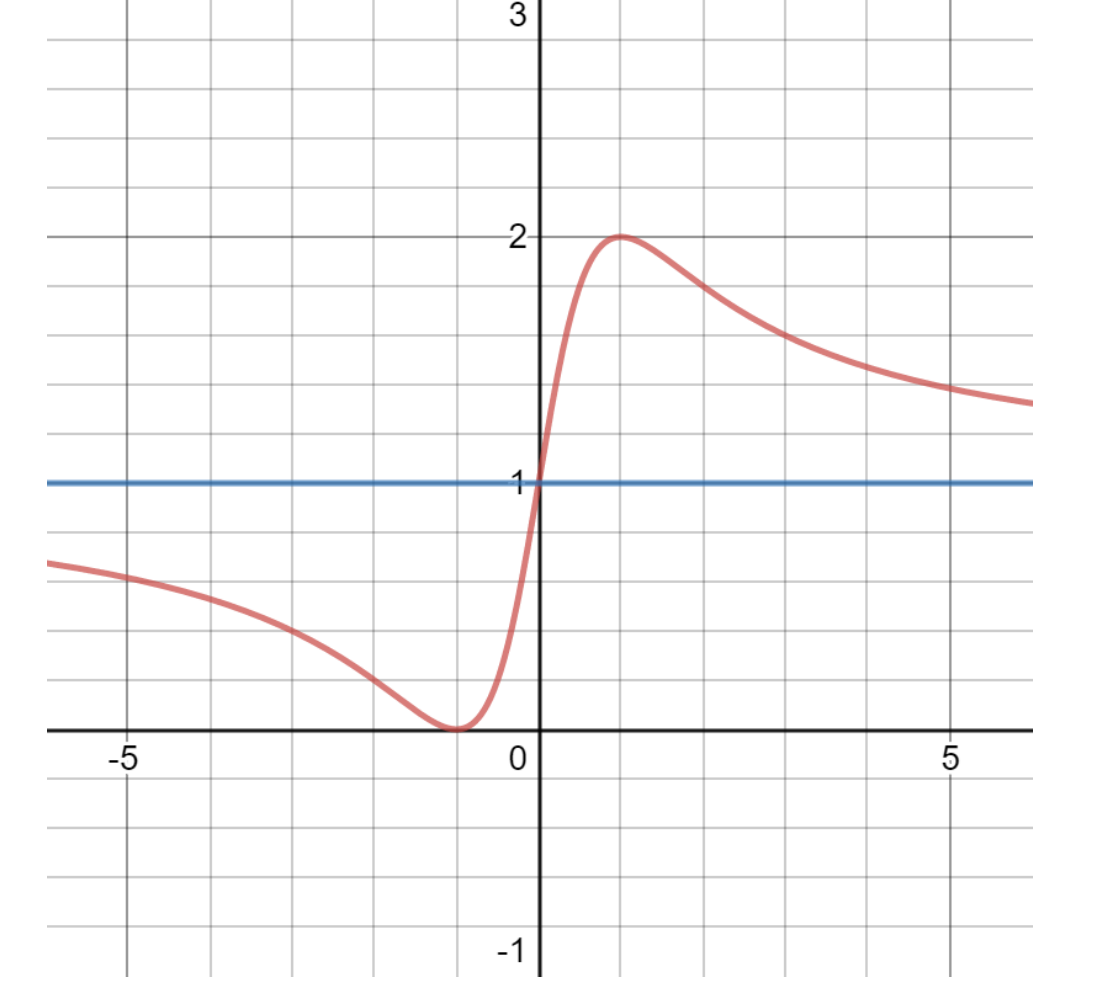
\includegraphics[width=0.38\linewidth,height=\textheight,keepaspectratio]{note-images/w4-sketch.png}\par
\vspace{3pt}
{\small \emph{Lecture 13, p.25.}\par}
\end{minipage}
\end{center}

Sketch order: domain, derivatives, critical points/signs, concavity,
asymptotes, key values. Here \(f(-x)=2-f(x)\): point symmetry about
\((0,1)\).

\Needspace{8\baselineskip}
\subsection{Three exercises}\label{three-exercises}

\textbf{Jordan.} Strict concavity of \(\sin\) on \([0,\pi/2]\) gives \[
\sin x>2x/\pi\qquad(0<x<\pi/2)
\] by comparison with the endpoint chord.

\textbf{Convex maximum.} Strict convexity on \([a,b]\) gives, for
\(a<x<b\), \(f(x)<\alpha f(a)+(1-\alpha)f(b)\le\max\{f(a),f(b)\}\).
Maximum only at endpoints (possibly both).

\textbf{Legendre roots.} \(P_n=(2^n n!)^{-1}D^n[(x^2-1)^n]\). Put
\(Q=(x^2-1)^n\). \[
Q^{(k)}(\pm1)=0\quad(0\le k<n).
\] Rolle gives one interior root of \(Q'\). If \(Q^{(k)}\) has \(k\)
interior roots, its endpoint zeros give \(k+1\) gaps, hence \(k+1\)
interior roots of \(Q^{(k+1)}\). Induct up to \(n\). Since
\(\deg Q^{(n)}=n\), all \(n\) roots are distinct and in \((-1,1)\).

\Needspace{8\baselineskip}
\subsection{Newton's method}\label{newtons-method}

Linearize at \(x_n\), solve for the tangent's zero: \[
f(x_n)+f'(x_n)(x-x_n)=0
\implies x_{n+1}=x_n-\frac{f(x_n)}{f'(x_n)}.
\] Need \(f'(x_n)\ne0\) at each step.

\begin{center}
\begin{minipage}{\linewidth}
\centering
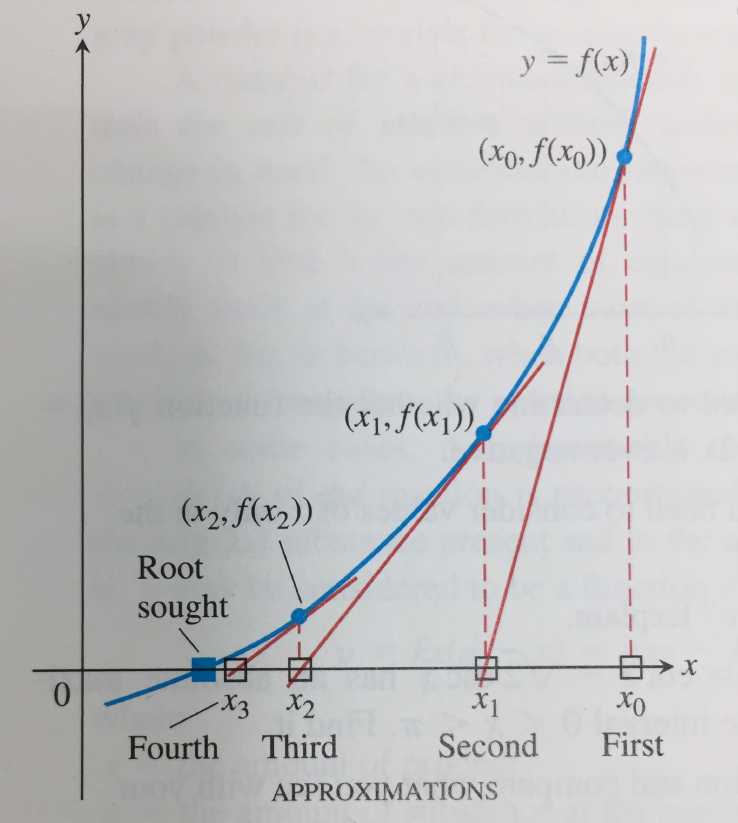
\includegraphics[width=0.34\linewidth,height=\textheight,keepaspectratio]{note-images/w4-newton.png}\par
\vspace{3pt}
{\small \emph{Lecture 13, p.35.}\par}
\end{minipage}
\end{center}

\textbf{Ex.1.2.47.} \(x^2=2\): \[
x_{n+1}=\tfrac12(x_n+2/x_n),\qquad
x_0=1,\ x_1=3/2,\ x_2=17/12,\ x_3=577/408.
\] For \(r=\sqrt2\), \(x_{n+1}-r=(x_n-r)^2/(2x_n)\). After the first
step, \(x_n\ge r\) and decreases; the positive limit solves
\(\ell=(\ell+2/\ell)/2\), so equals \(r\). Error is squared near the
root.

Failure examples: \(e^x\) gives \(x_{n+1}=x_n-1\) (no root).
\(\sqrt{|x|}\) gives \(x_{n+1}=-x_n\) for \(x_n\ne0\) (oscillation,
despite having a root).

\Needspace{10\baselineskip}
\section{Tutorial 3}\label{tutorial-3}

\Needspace{8\baselineskip}
\subsection{IVT / MVT}\label{ivt-mvt}

\Needspace{5\baselineskip}
\textbf{Q7.} \(F=\cos x-x\): \(F(0)>0>F(1)\) gives existence in
\((0,1)\) by IVT. \(F'=-\sin x-1<0\) there; two roots would contradict
MVT. Unique.

\Needspace{5\baselineskip}
\textbf{Q8.} Continuous, nonzero \(f\) on \([a,b]\):

\begin{enumerate}
\def\labelenumi{(\alph{enumi})}
\item
  Opposite signs would give a zero by IVT, so the sign is fixed.
\item
  EVT: \(m=\min|f|=|f(c)|>0\), hence \(|1/f|\le1/m\).
\item
  Open interval fails: \(f(x)=x\) on \((0,1)\).
\end{enumerate}

\Needspace{5\baselineskip}
\textbf{Q9.} MVT: \(\sin x-\sin y=\cos c\,(x-y)\), so \[
|\sin x-\sin y|\le|x-y|.
\] Uniform continuity: choose \(\delta=\varepsilon\), independent of
\(x,y\). More generally, \(|f'|\le M\) on an interval gives
\(|f(x)-f(y)|\le M|x-y|\) (Lipschitz).

\Needspace{8\baselineskip}
\subsection{Continuity and direct
estimates}\label{continuity-and-direct-estimates}

\Needspace{5\baselineskip}
\textbf{Q1.} \(g=x+b\) for \(x<0\), \(g=\cos x\) for \(x\ge0\).
Continuity at \(0\): \(b=1\). Then left/right derivatives \(1,0\), so no
\(b\) makes it differentiable.

\Needspace{5\baselineskip}
\textbf{Q3.} \(F=\varphi\) on \(\mathbb Q\), \(\psi\) otherwise;
\(\varphi,\psi\) continuous. \[
F\text{ continuous at }a\iff\varphi(a)=\psi(a).
\] Necessity: rational/irrational sequences approaching \(a\) force both
values to equal \(F(a)\). Sufficiency: if common value \(C\), choose a
common radius making both pieces within \(\varepsilon\) of \(C\). For
\(\sin x,-\sin x\), continuity points \(a=k\pi\).

\Needspace{5\baselineskip}
\textbf{Q10.} \((x^3-27)/(x^2-9)=(x^2+3x+9)/(x+3)\) off \(\pm3\). Limit
at \(3\) is \(9/2\), matching the assignment. At \(-3\), denominator
\(\to0\), numerator \(\to9\). Continuity set
\(\mathbb R\setminus\{-3\}\).

\Needspace{5\baselineskip}
\textbf{Q4(a).} If \(|f-A|,|g-B|<\varepsilon\), then \[
\begin{aligned}
\max(A,B)-\varepsilon&<\max(f,g)<\max(A,B)+\varepsilon,\\
\min(A,B)-\varepsilon&<\min(f,g)<\min(A,B)+\varepsilon.
\end{aligned}
\] Use \(\delta=\min(\delta_f,\delta_g)\): limits \(\max(A,B)\),
\(\min(A,B)\).

\Needspace{5\baselineskip}
\textbf{Q4(b).} Converse false: \(f=1_{\mathbb Q}\), \(g=1-f\). Max
\(1\), min \(0\); neither individual limit exists. The pieces exchange
roles.

\Needspace{5\baselineskip}
\textbf{Q2.} Rationalize twice, for \(0<|x|<1\): \[
\left|\frac{\sqrt{4+x}-2}{x}-\frac14\right|
=\frac{|x|}{4(\sqrt{4+x}+2)^2}\le\frac{|x|}{16}.
\] Limit \(1/4\); \(\delta=\min\{1,16\varepsilon\}\).

\Needspace{8\baselineskip}
\subsection{Q11: trigonometric limits}\label{q11-trigonometric-limits}
\[
\begin{aligned}
\text{(a)}\quad &\frac{\sin(\sin2h)}h
=\frac{\sin(\sin2h)}{\sin2h}\frac{\sin2h}{2h}\,2\to2,\\
\text{(b)}\quad &\frac{\sin4y\cot7y}{y\cot3y}
=\frac{\sin4y}{y}\frac{\sin3y}{\sin7y}\frac{\cos7y}{\cos3y}\to\frac{12}7,\\
\text{(c)}\quad &\frac{\tan2x-\sin2x}{x^3}
=\frac{\sin2x}{x}\frac{2\sin^2x}{x^2}\frac1{\cos2x}\to4,\\
\text{(d)}\quad &\frac{\cos^2x-\cos^2a}{x-a}
=-\sin(x+a)\frac{\sin(x-a)}{x-a}\to-\sin2a,\\
\text{(e)}\quad &\frac{\sqrt{1-\cos3x^2}}{1-\cos2x}
=\frac{\sqrt2|\sin(3x^2/2)|}{2\sin^2x}\to\frac{3\sqrt2}{4}.
\end{aligned}
\] In (c), factor exactly; first-order approximations cannot recover the
cubic term. In (e), keep the absolute value.

\Needspace{8\baselineskip}
\subsection{Q12: radii / thresholds}\label{q12-radii-thresholds}

\begin{enumerate}
\def\labelenumi{(\alph{enumi})}
\item
  \(x\to-1^+\): \((x+1)/|x+1|=1\) exactly. Any \(\delta>0\).
\item
  \(x\to+\infty\): \[
  \left|\frac{7x^2+2}{x^2+1}-7\right|=\frac5{x^2+1}<\frac5{x^2};\quad
  M=\max\{1,\sqrt{5/\varepsilon}\}.
  \]
\item
  By Q9, for \(x>2\), \[
  |\sin\sqrt{x+2}-\sin\sqrt{x-2}|
  \le\frac4{\sqrt{x+2}+\sqrt{x-2}}\le\frac4{\sqrt{x-2}}.
  \] Limit \(0\); \(M=2+16/\varepsilon^2\).
\item
  Put \(h=x-a>0\), \(a>0\). Rationalizing the first numerator term gives
  \[
  E(h)=\frac{\sqrt h}{(\sqrt{a+h}+\sqrt a)\sqrt{2a+h}}
  +\frac2{\sqrt{2a+h}}\to\sqrt{2/a}.
  \] For \(0<h<1\), \[
  |E(h)-2/\sqrt{2a}|\le\frac{\sqrt h}{2\sqrt2\,a}+\frac{h}{(2a)^{3/2}}
  \le C\sqrt h,
  \] where \(C=(2\sqrt2\,a)^{-1}+(2a)^{-3/2}\). Use
  \(\delta=\min\{1,(\varepsilon/C)^2\}\).
\end{enumerate}

\Needspace{8\baselineskip}
\subsection{Functional relations}\label{functional-relations}

\Needspace{5\baselineskip}
\textbf{Q5(a).} Fix \(x\ge0\). Periodicity gives \(f(x)=f(x+n)\to L\),
hence \(f(x)=L\).

\Needspace{5\baselineskip}
\textbf{Q5(b).} Counterexample \(f(x)=\sin\sqrt x\) on \([0,\infty)\):
bounded, continuous, and \[
|f(x+1)-f(x)|\le\frac1{\sqrt{x+1}+\sqrt x}\to0.
\] At \((\pi/2+2n\pi)^2\) values are \(1\); at \((3\pi/2+2n\pi)^2\),
\(-1\). No limit.

\Needspace{5\baselineskip}
\textbf{Q6: halving and telescoping.} Assume \(f(x)\to0\) and
\([f(2x)-f(x)]/x\to0\) as \(x\to0^+\). Given \(\varepsilon>0\), choose
\(0<\delta<1\) with \[
|f(2t)-f(t)|<\frac\varepsilon2t\qquad(0<t<\delta).
\] For \(0<x<\delta\), apply at \(t=x/2^k\): \[
\begin{aligned}
|f(x)-f(x/2^N)|
&\le\sum_{k=1}^N|f(x/2^{k-1})-f(x/2^k)|\\
&\le\frac{\varepsilon x}2\sum_{k=1}^N2^{-k}<\frac{\varepsilon x}2.
\end{aligned}
\] Fix \(x\), let \(N\to\infty\):
\(|f(x)|\le\varepsilon x/2<\varepsilon x\). Thus \(f(x)/x\to0\). Need
the first hypothesis to remove the last term (nonzero constants would
fail).

\Needspace{5\baselineskip}
\textbf{Q13.} For \(0\le x<1\), \(f(x)=f(x^{2^n})\to f(0)\) by
continuity at \(0\). At \(1\), no restriction: \(f=0\) on \([0,1)\),
\(f(1)=1\) is a counterexample. Continuity at \(1\) forces
\(f(1)=f(0)\).

\Needspace{5\baselineskip}
\textbf{Q14.} \(g(x)=f(x^2)\): \[
\lim_{x\to0}g(x)=L\iff\lim_{t\to0^+}f(t)=L.
\] Right to left: from radius \(\eta\) for \(f\), take
\(\delta=\sqrt\eta\). Left to right: from radius \(\delta\) for \(g\),
take \(0<t<\delta^2\), \(x=\sqrt t\).

Continuity of \(g\) need not give continuity of \(f\): \(f=0\) for
\(t\ge0\), \(1\) for \(t<0\) makes \(g\equiv0\).

\Needspace{5\baselineskip}
\textbf{Q15.} Additivity gives \(f(0)=0\) and \(f(a+h)-f(a)=f(h)\).
Continuity at \(0\) transports the same \(\varepsilon\)-\(\delta\)
estimate to every \(a\). In fact the radius is independent of \(a\).

\newpage

\Needspace{10\baselineskip}
\section{Lecture 14}\label{lecture-14}

\Needspace{8\baselineskip}
\subsection{Antiderivatives and the
constant}\label{antiderivatives-and-the-constant}

\Needspace{5\baselineskip}
\textbf{Definition 1.2.13.} \(F\) is an antiderivative of \(f\) on an
interval \(I\) if \(F'=f\) throughout \(I\). Always specify the
interval.

\Needspace{5\baselineskip}
\textbf{Theorem 1.2.14.} If \(F\) is one antiderivative on \(I\), all
others are \(F+C\).

Proof: \((G-F)'=0\) on the interval; MVT makes \(G-F\) constant. On
separate components the constants are independent. E.g. \[
\int x\,dx=\begin{cases}x^2/2+C_-,&-2<x<-1,\\x^2/2+C_+,&1<x<2.\end{cases}
\] \textbf{Definition 1.2.15.} \(\int f(x)\,dx\) is the family
\(\{F+C:C\in\mathbb R\}\) on the chosen interval, usually written
\(F(x)+C\). Not a single function until \(C\) is fixed.

Basic formulas (\(k\ne0\); work on intervals where the expressions are
defined): \[
\begin{array}{c|c@{\qquad}c|c}
f&\int f\,dx&f&\int f\,dx\\\hline
x^p\ (p\ne-1)&\dfrac{x^{p+1}}{p+1}+C&\sin kx&-\dfrac{\cos kx}{k}+C\\[5pt]
\cos kx&\dfrac{\sin kx}{k}+C&\sec^2kx&\dfrac{\tan kx}{k}+C\\[5pt]
\csc^2kx&-\dfrac{\cot kx}{k}+C&\sec kx\tan kx&\dfrac{\sec kx}{k}+C\\[5pt]
\csc kx\cot kx&-\dfrac{\csc kx}{k}+C&&
\end{array}
\] For arbitrary real \(p\), the power formula is used on \(x>0\);
extend only where the real powers make sense.

\textbf{Ex.1.2.48-50.} Integrate finite sums term by term. Useful
patterns: \[
\begin{aligned}
\int x^{-2}\,dx&=-x^{-1}+C\quad(x\ne0;\ C_-,C_+),\\
\int x^{1/3}\,dx&=\tfrac34x^{4/3}+C\quad(\mathbb R),\\
\int\sum_{k=0}^n a_k(x+b_k)^k\,dx
&=\sum_{k=0}^n\frac{a_k(x+b_k)^{k+1}}{k+1}+C,\\
\int\sum_{k=0}^n a_kx(x^2+b_k)^k\,dx
&=\sum_{k=0}^n\frac{a_k(x^2+b_k)^{k+1}}{2(k+1)}+C,\\
\int\sum_{k=1}^n[a_k\cos kx+b_k\sin kx]\,dx
&=\sum_{k=1}^n\frac{a_k\sin kx-b_k\cos kx}{k}+C.
\end{aligned}
\] Also \(\int\sqrt[k]{x+a_k}\,dx=\frac{k}{k+1}(x+a_k)^{(k+1)/k}+C\) on
its real intervals, and \(\int(x+b_k)^{-k}dx=(x+b_k)^{1-k}/(1-k)+C\) for
\(k\ge2\). Check by differentiating.

\Needspace{8\baselineskip}
\subsection{Joining the pieces}\label{joining-the-pieces}

\textbf{Ex.1.2.51.} A compact answer: \[
\int|x-a|\,dx=\tfrac12(x-a)|x-a|+C\qquad(x\in\mathbb R).
\] At \(a\), the quotient is \(|h|/2\to0\). Splitting into two formulas
does not give two free constants if the antiderivative is required on
all of \(\mathbb R\).

\textbf{Ex.1.2.52(a).} For \(f(x)=\min\{1,|x|\}\), \[
F(x)=C+\begin{cases}
x+1/2,&x\le-1,\\
x|x|/2,&-1\le x\le1,\\
x-1/2,&x\ge1.
\end{cases}
\] Values match at \(\pm1\); derivative there is \(1\). At \(0\),
derivative \(0\). Hence \(F'=f\) on \(\mathbb R\).

\textbf{Ex.1.2.52(b,c): a jump.} For either step function
\(1_{[0,\infty)}\) or \(1_{(0,\infty)}\), no antiderivative exists on an
open interval about \(0\): continuity of a proposed primitive joins a
constant on the left to \(x+C\) on the right, giving one-sided slopes
\(0,1\).

On \(\mathbb R\setminus\{0\}\), however, the primitives are \(C_-\) for
\(x<0\) and \(x+C_+\) for \(x>0\), with independent constants. Removing
the joining point changes the problem.

\textbf{Ex.1.2.53.} For \(k\in\mathbb Z\) and \(k\pi\le x\le(k+1)\pi\),
\[
\int|\sin x|\,dx=C+2k+1-(-1)^k\cos x.
\] Both adjacent formulas give \(C+2k\) at \(x=k\pi\); both derivatives
there are \(0\). Thus this is one primitive on \(\mathbb R\). Its value
increases by \(2\) each half-period; the primitive is not periodic.

\Needspace{10\baselineskip}
\section{Lecture 15}\label{lecture-15}

\Needspace{8\baselineskip}
\subsection{Sums, partitions, tags}\label{sums-partitions-tags}
\[
\sum_{k=1}^n k=\frac{n(n+1)}2,\quad
\sum_{k=1}^n k^2=\frac{n(n+1)(2n+1)}6,\quad
\sum_{k=1}^n k^3=\left[\frac{n(n+1)}2\right]^2.
\] Two standard finite sums: \(\sum_{k=1}^n2^{-k}=1-2^{-n}\) and
\(\sum_{k=1}^n[k(k+1)]^{-1}=1-(n+1)^{-1}\).

\Needspace{5\baselineskip}
\textbf{Definition.} A partition \(P\) of \([a,b]\): \[
a=x_0<x_1<\cdots<x_n=b,\quad
\Delta x_k=x_k-x_{k-1},\quad \|P\|=\max_k\Delta x_k.
\] Choose tags \(c_k\in[x_{k-1},x_k]\). The Riemann sum is \[
S(f,P,\mathbf c)=\sum_{k=1}^n f(c_k)\Delta x_k.
\]

\begin{center}
\begin{minipage}{\linewidth}
\centering
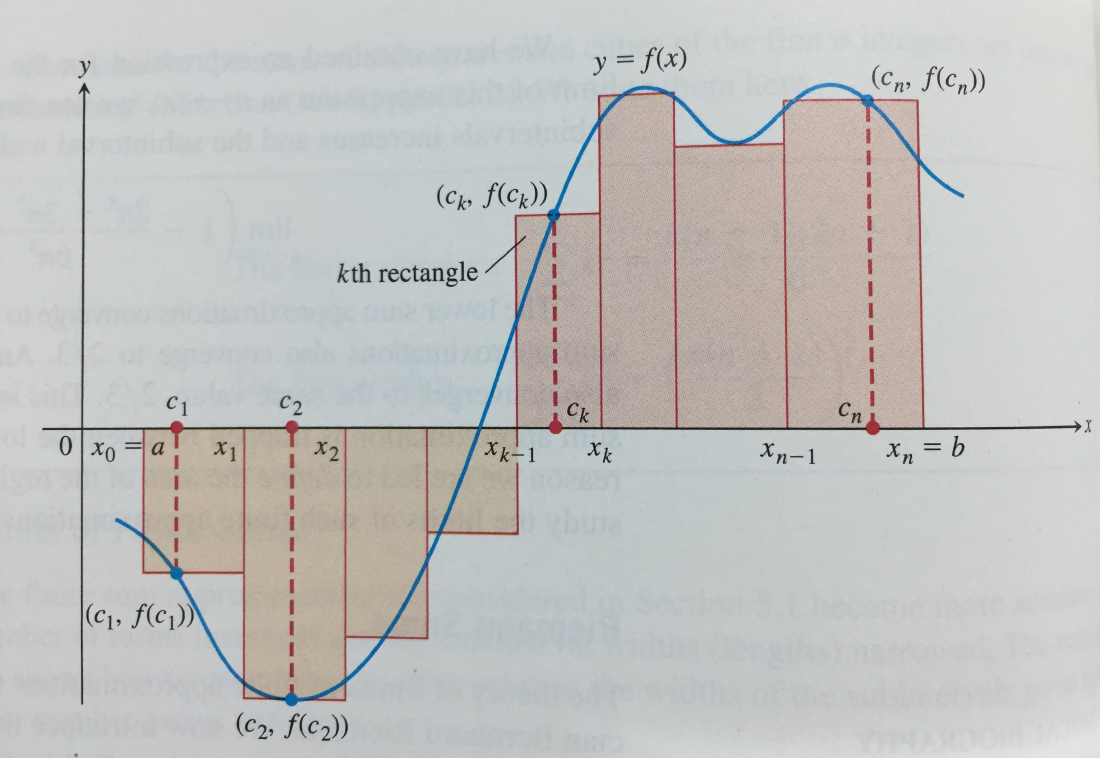
\includegraphics[width=0.52\linewidth,height=\textheight,keepaspectratio]{note-images/w5-riemann.png}\par
\vspace{3pt}
{\small \emph{Lecture 15, p.12. Negative heights contribute negative terms.}\par}
\end{minipage}
\end{center}

Equal widths \(\Delta=(b-a)/n\): left, midpoint and right tags are
\(a+(k-1)\Delta\), \(a+(k-1/2)\Delta\), \(a+k\Delta\).

For bounded \(f\), let \(m_k=\inf_{[x_{k-1},x_k]}f\),
\(M_k=\sup_{[x_{k-1},x_k]}f\). Then \[
L(f,P)=\sum m_k\Delta x_k\le S(f,P,\mathbf c)\le\sum M_k\Delta x_k=U(f,P).
\]

\begin{center}
\begin{minipage}{\linewidth}
\centering
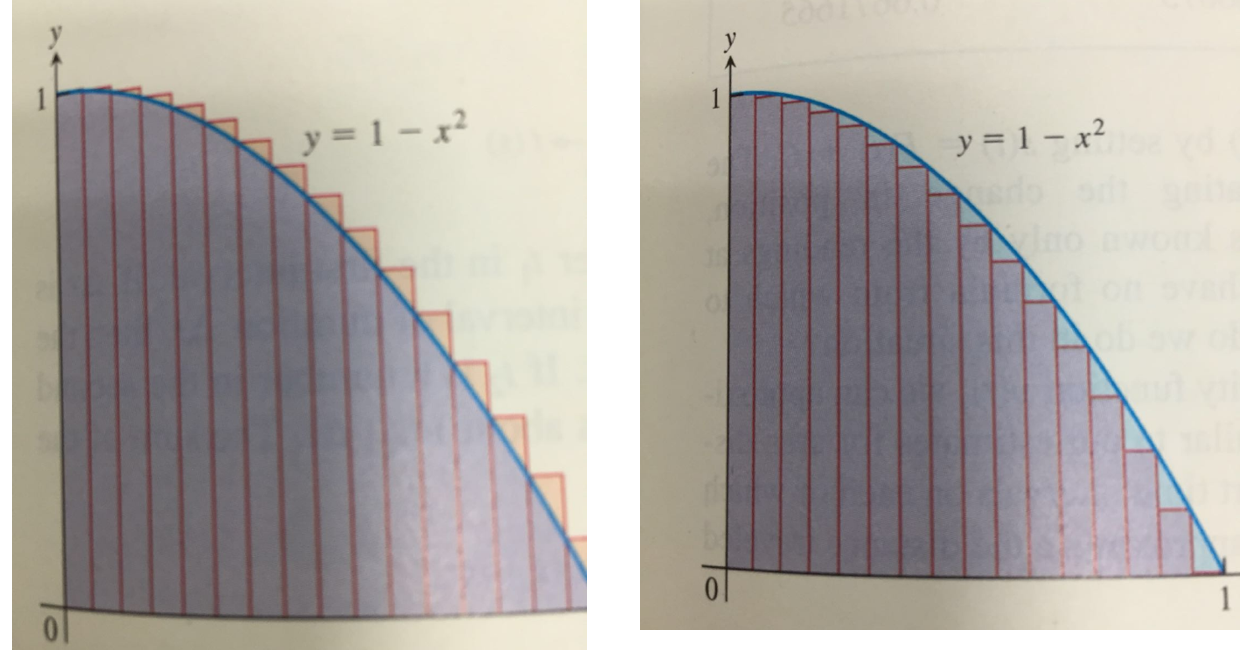
\includegraphics[width=0.57\linewidth,height=\textheight,keepaspectratio]{note-images/w5-upper-lower.png}\par
\vspace{3pt}
{\small \emph{Lecture 15, pp.4-5. Upper / lower rectangles for \(1-x^2\) on
\([0,1]\).}\par}
\end{minipage}
\end{center}

\Needspace{8\baselineskip}
\subsection{The limit must ignore the
choices}\label{the-limit-must-ignore-the-choices}

\Needspace{5\baselineskip}
\textbf{Definition (Riemann integral).} \(f:[a,b]\to\mathbb R\) is
integrable with integral \(J\) if \[
\forall\varepsilon>0\ \exists\delta>0\ \forall P\ \forall\mathbf c:
\qquad \|P\|<\delta\implies|S(f,P,\mathbf c)-J|<\varepsilon.
\] Write \(J=\int_a^b f(x)\,dx\). This is a number; \(\int f(x)\,dx\) is
a family of functions.

\begin{itemize}
\tightlist
\item
  Need \textbf{all} sufficiently fine partitions and \textbf{all} tags.
  One convergent sequence of sums is not enough to prove integrability.
\item
  \(n\to\infty\) does not imply \(\|P\|\to0\): keep \([0,1/2]\) as one
  cell and subdivide \([1/2,1]\) more and more.
\item
  Finite endpoint changes do not affect \(J\): the change in a sum is at
  most \((|\Delta f(a)|+|\Delta f(b)|)\|P\|\).
\end{itemize}

\textbf{Ex.2.1.1.} For \(x^2\) on \([0,1]\), right sums give \[
\frac1{n^3}\sum_{k=1}^n k^2
=\frac16(1+1/n)(2+1/n)\to\frac13.
\] To check arbitrary partitions/tags, use \(F=x^3/3\). MVT on each cell
gives \(\Delta F=\xi_k^2\Delta x_k\). Therefore \[
\left|S-\frac13\right|
\le\sum|c_k^2-\xi_k^2|\Delta x_k
\le2\|P\|\sum\Delta x_k=2\|P\|.
\] So \(\delta=\varepsilon/2\) works. Likewise the right sums for
\(1-x^2\) tend to \(2/3\): \[
\frac1n\sum_{k=1}^n[1-(k/n)^2]
=1-\frac16(1+1/n)(2+1/n)\to\frac23.
\]

\Needspace{10\baselineskip}
\section{Tutorial (Homework 3)}\label{tutorial-homework-3}

This is the new five-page sheet, not the earlier Tutorial 3.

\Needspace{8\baselineskip}
\subsection{Q1: limits}\label{q1-limits}

\begin{enumerate}
\def\labelenumi{(\alph{enumi})}
\item
  \(s_n=\sum_{k=1}^n(1/k-1/(k+1))=1-1/(n+1)\to1\). Given
  \(\varepsilon>0\), choose an integer \(N>1/\varepsilon\);
  \(n>N\Rightarrow|s_n-1|<\varepsilon\).
\item
  Put \(a=1+t\), \(t>0\). For \(n\ge2\), \[
  a^n\ge\binom n2t^2\implies0\le\frac n{a^n}\le\frac2{(n-1)t^2}\to0.
  \] Choose an integer \(N>\max\{2,1+2/(\varepsilon t^2)\}\).
\item
  Cancel before taking the limit: \[
  \frac1{1-x}-\frac3{1-x^3}=-\frac{x+2}{x^2+x+1}\to-1.
  \] For \(0<|x-1|<1/2\), error \(=|x-1||x+1|/(x^2+x+1)\le(5/2)|x-1|\).
  Use \(\delta=\min\{1/2,2\varepsilon/5\}\).
\item
  Let \(s=\sqrt{1+x}+\sqrt{1-x}\). Rationalize twice: \[
  \frac{s-2}{x^2}=-\frac2{(\sqrt{1-x^2}+1)(s+2)}\to-\frac14.
  \]
\item
  \(\cos2x-4\cos x+3=2(1-\cos x)^2=8\sin^4(x/2)\); dividing by \(x^4\)
  gives limit \(1/2\).
\end{enumerate}

\Needspace{8\baselineskip}
\subsection{Q2-Q4: auxiliary functions and
asymptotes}\label{q2-q4-auxiliary-functions-and-asymptotes}

\Needspace{5\baselineskip}
\textbf{Q2(a).} \(f\in C[0,1]\), differentiable inside, \(f(0)=0\),
\(f(1)=1\). IVT gives \(t\in(0,1)\) with \(f(t)=1/2\). MVT on \([0,t]\),
\([t,1]\) gives \(0<\xi<t<\eta<1\) and \[
f'(\xi)=\frac1{2t}>0,\quad f'(\eta)=\frac1{2(1-t)}>0;\qquad
\frac1{f'(\xi)}+\frac1{f'(\eta)}=2.
\]

\Needspace{5\baselineskip}
\textbf{Q2(b).} Set \(H(x)=(1-x)f(x)\). Since \(H(0)=H(1)=0\), Rolle
gives \((1-c)f'(c)-f(c)=0\). The product is chosen to produce the
requested derivative.

\Needspace{5\baselineskip}
\textbf{Q3(a).} \(f=\sqrt{x^2+2x}-x\), domain
\((-\infty,-2]\cup[0,\infty)\): \[
\begin{aligned}
x\to+\infty:&\quad f=\frac2{\sqrt{1+2/x}+1}\to1,\\
x\to-\infty:&\quad f-(-2x-1)=\sqrt{x^2+2x}+x+1\to0.
\end{aligned}
\] For the second line, \(\sqrt{x^2+2x}+x=2x/(\sqrt{x^2+2x}-x)\to-1\).
Horizontal \(y=1\) on the right; oblique \(y=-2x-1\) on the left.
Endpoint values finite, so no vertical asymptote. Use
\(\sqrt{x^2}=|x|\).

\Needspace{5\baselineskip}
\textbf{Q3(b).} \(g=\sqrt{x^2+1}/x\): limits \(1,-1\) at
\(+\infty,-\infty\); limits \(+\infty,-\infty\) at \(0^+,0^-\).
Horizontal lines \(y=1,-1\), vertical \(x=0\); no oblique lines.

\Needspace{5\baselineskip}
\textbf{Q3(c).} \[
h=\frac{(x-1)(x^2+1)}{(x-1)(x-2)}=x+2+\frac5{x-2}\quad(x\ne1,2).
\] Vertical \(x=2\), oblique \(y=x+2\) at both infinities. \(x=1\) is a
removable hole (limit \(-2\)), not a vertical asymptote. No horizontal
line.

\Needspace{5\baselineskip}
\textbf{Q4.} As in Tutorial 3, Q8: IVT fixes the sign; EVT gives
\(m=\min|f|>0\), hence \(|1/f|\le1/m\). On \((0,1)\), \(f(x)=x\) shows
the open-interval conclusion fails.

\Needspace{8\baselineskip}
\subsection{Q5-Q8: derivatives and
extrema}\label{q5-q8-derivatives-and-extrema}

\Needspace{5\baselineskip}
\textbf{Q5.} \(F=ax+b\) for \(x<0\), \(F=\cos x\) for \(x\ge0\).

\begin{enumerate}
\def\labelenumi{(\alph{enumi})}
\item
  Continuity: \(b=1\), any \(a\).
\item
  One-sided derivatives \(a,0\); differentiable iff \((a,b)=(0,1)\),
  then \(F'(0)=0\).
\item
  For these values, \(F'=0\) on the left, \(-\sin x\) on the right;
  continuous at \(0\). But the one-sided difference quotients of \(F'\)
  tend to \(0,-1\), so \(F''(0)\) does not exist.
\end{enumerate}

\Needspace{5\baselineskip}
\textbf{Q6(a).} For \(y=\sin(x^2)/\sqrt{1+x^2}\), \[
y'=\frac{2x\cos(x^2)}{\sqrt{1+x^2}}-\frac{x\sin(x^2)}{(1+x^2)^{3/2}}.
\] \textbf{Q6(b).} \(y=\arcsin[2x/(1+x^2)]\): \[
\sqrt{1-\left(\frac{2x}{1+x^2}\right)^2}=\frac{|1-x^2|}{1+x^2},\qquad
y'=\begin{cases}2/(1+x^2),&|x|<1,\\-2/(1+x^2),&|x|>1.\end{cases}
\] Not differentiable at \(\pm1\): left/right slopes are \(-1,1\) at
\(-1\) and \(1,-1\) at \(1\). The square root needs the absolute value.

\Needspace{5\baselineskip}
\textbf{Q6(c).} Leibniz, \(P=(1+x^2)\cos x\), \(n\ge2\): \[
\begin{aligned}
P^{(n)}={}&(1+x^2)\cos(x+n\pi/2)+2nx\cos(x+(n-1)\pi/2)\\
&+n(n-1)\cos(x+(n-2)\pi/2).
\end{aligned}
\]

\Needspace{5\baselineskip}
\textbf{Q7.} \(x^2+xy+y^2=3\), \(y(1)=1\): \[
\begin{aligned}
2x+y+(x+2y)y'&=0\implies y'(1)=-1,\\
2+2y'+2(y')^2+(x+2y)y''&=0\implies y''(1)=-2/3.
\end{aligned}
\] Tangent \(y-1=-(x-1)\); normal \(y-1=x-1\). Linearization
\(L(x)=2-x\), so \(y(1.02)\approx0.98\).

\Needspace{5\baselineskip}
\textbf{Q8.} \(f=x^3|x-1|\) on \([-1,2]\): \[
f'=\begin{cases}x^2(3-4x),&x<1,\\x^2(4x-3),&x>1.\end{cases}
\qquad
\begin{array}{c|ccccc}
x&-1&0&3/4&1&2\\\hline
f(x)&-2&0&27/256&0&8
\end{array}
\] Interior critical points \(0,3/4,1\). Signs of \(f'\): \(+\) up to
\(3/4\) (except zero at \(0\)), then \(-\) up to \(1\), then \(+\).
Local max at \(3/4\), local min at \(1\); \(0\) is neither. Absolute min
\(-2\) at \(-1\), max \(8\) at \(2\).

\Needspace{8\baselineskip}
\subsection{Q9-Q11: what derivative bounds
force}\label{q9-q11-what-derivative-bounds-force}

\Needspace{5\baselineskip}
\textbf{Q9(a).} Differentiable \(f\) on an open interval \(I\): \[
|f'|\le M\iff|f(x)-f(y)|\le M|x-y|\quad(x,y\in I).
\] Forward: MVT. Reverse: divide by \(|h|\), then let \(h\to0\).

\Needspace{5\baselineskip}
\textbf{Q9(b).} If \(f(b)-f(a)=M(b-a)\), for \(a\le x\le b\) the
Lipschitz bounds give \[
f(b)-M(b-x)\le f(x)\le f(a)+M(x-a).
\] The two bounds are equal. Thus \(f(x)=f(a)+M(x-a)\) throughout
\([a,b]\).

\Needspace{5\baselineskip}
\textbf{Q9(c).} From \(|g(x)-g(y)|\le C|x-y|^2\), \[
\left|\frac{g(x+h)-g(x)}h\right|\le C|h|\to0.
\] Hence \(g'=0\) and \(g\) is constant by MVT. With exponent \(1\),
\(g(x)=x\) is a counterexample.

\Needspace{5\baselineskip}
\textbf{Q10.} Zeros \(x_n\ne c\), \(x_n\to c\); \(f\) differentiable at
\(c\).

\begin{enumerate}
\def\labelenumi{(\alph{enumi})}
\item
  Continuity gives \(f(c)=0\); along \(x_n\),
  \([f(x_n)-f(c)]/(x_n-c)=0\), so \(f'(c)=0\).
\item
  If \(f\) is differentiable near \(c\) and \(f''(c)\) exists, Rolle
  between \(x_n,c\) gives \(z_n\ne c\) with \(f'(z_n)=0\) and
  \(z_n\to c\). Therefore \(f''(c)=\lim[f'(z_n)-f'(c)]/(z_n-c)=0\).
\end{enumerate}

\Needspace{5\baselineskip}
\textbf{Q11 (Darboux property).} Given \(f'(a)<\lambda<f'(b)\), set
\(H=f-\lambda x\). Then \(H'(a)<0<H'(b)\), so neither endpoint minimizes
\(H\) on \([a,b]\). EVT + Fermat gives an interior minimum \(c\) with
\(H'(c)=0\), i.e.~\(f'(c)=\lambda\).

No continuity of \(f'\) used. A derivative may oscillate, but cannot
have a jump.

\Needspace{8\baselineskip}
\subsection{Supplementary exercises}\label{supplementary-exercises}

\textbf{S1: interpolation error.} \(f\in C[a,b]\), twice differentiable
inside, \(|f''|\le M\). Let \(L\) be the chord interpolant and set \[
E=f-L,\qquad q(x)=\frac M2(x-a)(b-x).
\] Both \(E\) and \(q\) vanish at the endpoints. Since \[
(E-q)''=f''+M\ge0,\qquad (E+q)''=f''-M\le0,
\] the chord inequalities give \(E-q\le0\) and \(E+q\ge0\). Thus \[
|f(x)-L(x)|\le\frac M2(x-a)(b-x)\le\frac{M(b-a)^2}8.
\] Smallest constant \(K=1/8\): equality at the midpoint for
\(f(x)=\frac M2(x-a)(x-b)\), whose chord is zero.

\textbf{S2: a primitive vs.~an integral.} \[
g_\lambda(x)=\begin{cases}2x\sin(1/x)-\cos(1/x),&x\ne0,\\\lambda,&x=0.\end{cases}
\] (a) Put \(F(x)=x^2\sin(1/x)\) off \(0\), \(F(0)=0\). We know
\(F'(0)=0\); \(F'=g_0\) everywhere. If \(G'=g_\lambda\), then off \(0\),
\(G=F+C_\pm\). Continuity at \(0\) forces one common constant, hence
\(G'(0)=0\). Therefore \[
\lambda=0\text{ only};\qquad\text{all primitives: }F+C.
\]

\begin{enumerate}
\def\labelenumi{(\alph{enumi})}
\setcounter{enumi}{1}
\tightlist
\item
  All \(\lambda\) are Riemann integrable on \([-1,1]\). Prove it for
  arbitrary tagged sums, using MVT rather than an integration formula.
\end{enumerate}

Set \(J=F(1)-F(-1)=2\sin1\) and \(B=3+|\lambda|\), so
\(|g_\lambda|\le B\) and \(|F'|\le3\) on \([-1,1]\). Given
\(\varepsilon>0\), choose \[
r=\min\left\{\frac14,\frac{\varepsilon}{16(B+3)}\right\},\quad
A=2+2/r+1/r^2,\quad \delta=\min\{r,\varepsilon/(4A)\}.
\] For any \(\|P\|<\delta\), MVT gives
\(\Delta F_k=g_0(\xi_k)\Delta x_k\), so \[
S(g_\lambda,P,\mathbf c)-J
=\sum_k[g_\lambda(c_k)-g_0(\xi_k)]\Delta x_k.
\] Split cells into two groups:

\begin{itemize}
\tightlist
\item
  Cells meeting \([-r,r]\): total width \(\le2r+2\|P\|<4r\). Error
  \(\le4r(B+3)\le\varepsilon/4\).
\item
  Other cells: \(c_k,\xi_k\) lie on the same side, with \(|x|\ge r\).
  Here \(|g_0'|\le A\), so their total error is
  \(\le A\|P\|\sum\Delta x_k<2A\delta\le\varepsilon/2\).
\end{itemize}

Total error \(<\varepsilon\), independently of all tags. Hence \[
\int_{-1}^1g_\lambda(x)\,dx=2\sin1\qquad(\lambda\in\mathbb R).
\] Changing one value preserves the integral, but can destroy the
existence of a primitive.
\end{document}
